\subsection{Descripción del problema.}

\vspace*{0.3cm}



\textbf{Introducción al problema} \newline


\vspace*{0.3cm}

%Estamos en el año 2048 y el pabellon 0+infinito es todo un exito. Los alumnos de algoritmos 3. Los alumnos de algoritmos 3 estan muy contentos porque van a cursar este cuatrimestre en un aula que está en el piso N, que es el más alto de todos. Con los avances de la ciencia y tegnologia, escaleras y ascensores han quedado obsoletos, y la forma de subir de un piso a otro es a través de portales. El nuevo pabellón tiene P portales, cada uno de los cuales permite subir de un piso A a un piso más alto B(para bajar de piso hay que tirarse con un paracaídas al piso 0 y luego volver a subir de ser necesario). 

%Uno de los alumnos, que estaba cursando en el segurno cuatrimestre de 2015 y fue congelado por el método de criogenia, acaba de ser descongelado y no puede creer lo bueno que están estos portales, algo que en su epoca no existía . Luego de completar todos los censos de estudiantes desde el año 2015 en adelate, este alumno quiere usar la mayor cantidad de portales posibles para legar al piso N y así seguir cursando Algoritmos III. Diseñar un algoritmo de complejidad $O(N^2)$ para calcular la mayor cantidad de portales que puede utilizar el alumno para subir desde planta baja al piso N (sin tirarse nunca con paracaídas). Se asegura que en toda instancia del problema es posible realizar el recorrido deseado, y que no hay más de un portal que comunique el mismo para de pisos. 

Estamos ubicados en el año 2048 y el pabellón 0+infinito es todo un éxito. Ese cuatrimestre les toco a los alumnos de algoritmos III cursar en el ultimo piso (piso N) y están muy contentos por eso.\newline
Con el avance de la ciencia y tecnología los ascensores, escaleras han quedado muy antiguos(obsoletos), es su lugar se han usado portales que \underline{sirven solamente para subir} de un piso a otro. \newline 
Este actual pabellón tiene P portales, cada uno de estos permite subir desde un piso A a un piso B, donde piso piso A es menor que el piso B.
La única manera de bajar de un piso es tirándose con paracaídas, el cual llega hasta el piso 0. Por lo cual si nos equivocamos en la elección deberemos intentarlos nuevamente desde el inicio(planta baja).\newline 
Uno de los alumnos, que estaba cursando en el segundo cuatrimestre de 2015, fue congelado por el método de criogenia. Este alumno fue descongelado y esta asombrado por el imponente edificio 0+infinito, y no puede creer lo bueno que están los portales(en su época sólo existían ascensores y escaleras). Luego de cumplir con sus obligaciones de completar los censos de 2015 hasta 2048, este alumno quiere quiere usar la mayor cantidad de portales para llegar al piso N y así llegar a cursar Algoritmos III. \newline

\begin{figure}[H]
  \begin{center}
      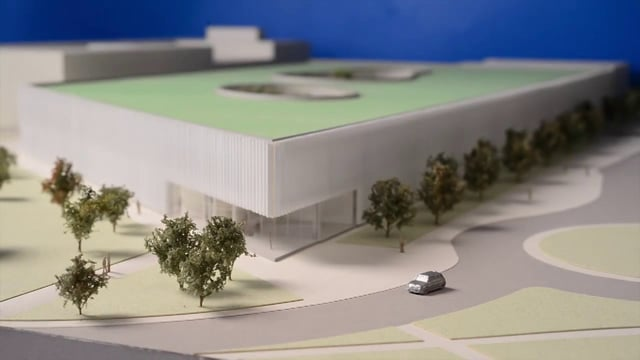
\includegraphics[scale=0.50]{imagenes/cero+infinito2.jpg}
  \end{center}
  \caption{Maqueta de edificio cero+infinito}
\end{figure}

\textbf{Problema a solucionar} \newline

Nuestro objetivo es diseñar un algoritmos de complejidad $O(N^2)$  para calcular la mayor cantidad de portales que puede utilizar este alumno para lograr subir desde planta baja hasta el piso N(no esta de mas decir que alumno no debería tirarse en paracaídas durante el trayecto).
Nos aseguran que en toda instancia del problema se podrá hacer el recorrido deseado y que no hay mas de un portal que comunique el mismo par de pisos.  

%%%%%% Informe anterior mal redactado %%%%

%El siguiente problema que presentaremos bien puede ser una situación que se nos presente en el a corto, mediano o largo plazo en la querida Facultad de Ciencias exacta y naturales. Cómo es sabido desde hace muy poco tiempo, se construirá un edificio el cual sera bautizado con el nombre Pabellón 0+infinito. Este edificio contendrá aulas, bibliotecas, oficinas, etc. Tendrá una cierta cantidad de pisos, que los alumnos, docentes, y otras personas deberán atravesar para llegar a sus respectivos lugares.

%\begin{figure}[H]
%  \begin{center}
%      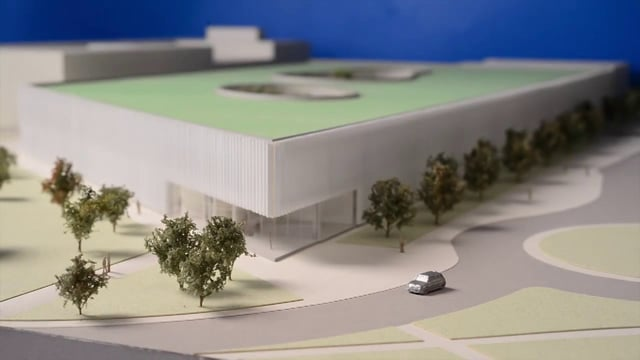
\includegraphics[scale=0.50]{imagenes/cero+infinito2.jpg}
%  \end{center}
%  \caption{Maqueta de edificio cero+infinito}
%\end{figure}



%Un alumno fue congelado por el método de criogenia en el año 2016, ahora es 2048 y este alumno es descongelado.
%El alumno se asombra de que se halla logrado construir el pabellón cero+infinito. Fue tanto su asombro que desea recorrer el edificio antes de ir a cursar algoritmos III. Este edificio cuenta con portales futuristas que comunican dos pisos distintos. 

%\newline
%\textbf{Problema a solucionar: }
%\newline

%El pabellón cero+infinito cuenta con $N$ pisos. 
%El tema es que los pisos están comunicado por $P$ portales, que van de un piso $A$ a otro $B$, dónde el piso $A$ es menor estricto que el piso $B$, osea los portales sólo van de hacia arriba. Y para bajar de los pisos se usan paracaídas que bajan hasta el suelo del pabellón(osea el piso 0), de modo tal que si el estudiante no llega al piso $N$, tendrá que volver a intentarlo. El objetivo del estudiante suba de una sola vez al último piso, atravesando la máxima cantidad de portales posibles. \newline


En los siguientes ejemplos se describirán algunos input del problema que se desea solucionar.
Notar que las columnas indican el piso inicial y final que une el portal, donde piso inicial es la base de la columna y piso final es el tope de la columna. \newline
 
 Ejemplo 1: \newline
 
\begin{figure}[htb]
  \centering
   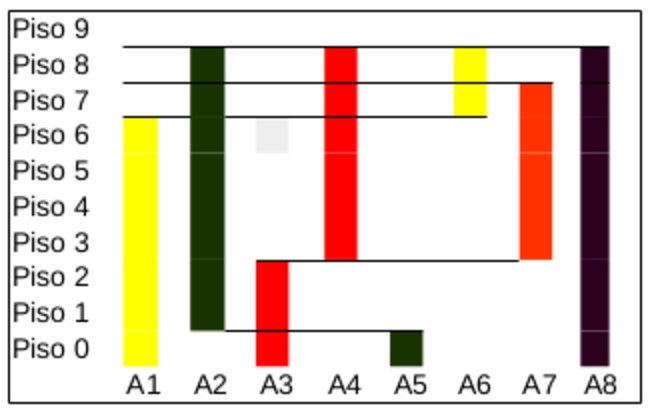
\includegraphics[scale=0.25]{imagenes/problema1Imagen1.jpg}
  \caption{Ejemplo 1}
\end{figure} 



En esta figura tenemos un conjunto de duplas, donde la primer componente de la dupla es el piso inicial, la segunda es el piso llegada: \newline

\begin{itemize}
    \item Input_1: 10 pisos y $\{(0,7),(1,9),(0,3),(3,9),(7,9),(3,8),(0,9)\} $ portales (ver imagen).
    \item Output_1: 2 
\end{itemize}
El output es 2 pues podemos usar dos portales como máximo para llegar al piso nueve(acordarse que siempre arrancamos del piso cero ). Por ejemplo en la figura los portales pueden ser cualquiera de estas tuplas $(A1,A6),(A3,A4)$ ó $(A5,A6)$.
\newline


Ejemplo 2 y 3:


\begin{figure}[H]
   \centering 
      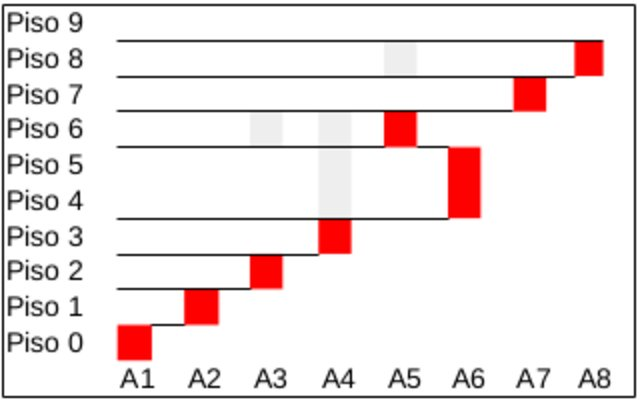
\includegraphics[scale=0.25]{imagenes/problema1Imagen2.jpg}
      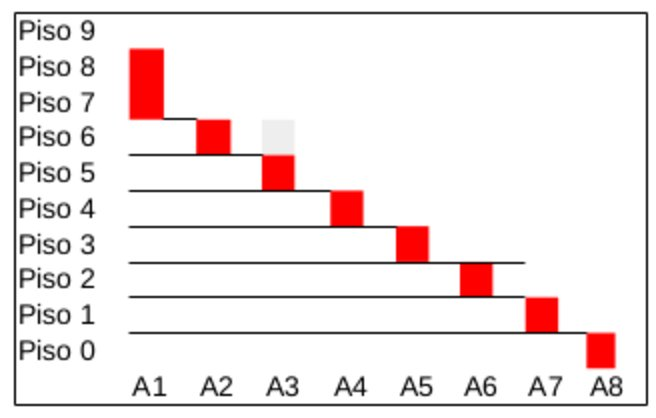
\includegraphics[scale=0.25]{imagenes/problema1Imagen3.jpg}
 \caption{ejemplo 2 y 3}
\end{figure}



\begin{itemize}
    \item Input_2: 10 pisos y $\{(0,1),(1,2),(2,3),(3,4),(6,7),(4,6),(7,8),(8,9)\}$ portales(ver imagen). 
    \item Input_3: 10 pisos y $\{(7,9),(6,7),(5,6),(4,5),(3,4),(2,3),(1,2),(0,1)\}$ portales(ver imagen)
    \item Output_2: 8 , pues debo usar todos los portales. en el siguiente orden \textbf{A1, A2, A3, A4, A6, A5, A7, A8}.  
    \item Output_3: 8 , pues debo usar también todos los portales(mirar figura), en el siguiente orden \textbf{A8, A7, A6, A5, A4, A3, A2, A1}.
\end{itemize}

%	\begin{figure}[htb]
%  \begin{center}
%      \includegraphics[scale=0.25]{imagenes/red-ferroviaria.jpg}
%	  \end{center}
% \caption{ejemplo}
%\end{figure}

\newpage
\subsection{Desarrollo de la idea y pseudocódigo.}

\vspace*{0.3cm}

%\textbf{completar.}
\textbf{}
Para la resolución de este ejercicio nos basamos el la técnica programación dinámica(en nuestro caso usamos bottom up). Lo que hacemos es crear una matriz $M$ de tamaño $nxn$ a la cual llenaremos inicialmente con 0 (ver pseudocódigo linea 2). Sea el elemento contenido en la posición de la  matriz M[i][j], denotamos con i a las filas, y j a las columnas. \newline
Hablemos un poco sobre la matriz y su contenido. Sean $ 0 \leq i \leq j \leq n-1 $: \newline
\begin{itemize}
	\item Solo usaremos la diagonal superior de la matriz.
	\item Si $ M[i][j] = 0 $ quiere decir que no hay forma de llegar él desde el piso $i$ al piso $j$.% pero no que no hay forma de llegar a él tomando mas de un portal.
	\item Si $ M[i][j] = 1 $ quiere decir que existe un portal que va del piso $i$ al piso $j$
	\item Por restricciones del problema se sabe que no exiten portales que unan piso $i$ con piso $i$, osea inicialmente todo $M[i][i] = 0$.  Eventualmente va a cambiar, para todo $i > 0$, y su contenido va a terminar siendo, la maxima cantidad de portales que se puede tomar para llegar a ese piso $i$, desde el primer piso.
%	\item Dentro de la matriz también guardaremos el máximo obtenido hasta el momento preferentemente en  la posición M[i][i] con $0 \leq i \leq n-1 $.
\end{itemize}

Luego recorreremos los portales, y para cada portal P, que va desde el piso $i$ al piso $j$, con $i < j$, se le pondrá en la matriz, en la posición $i,j$ un 1 (Ver linea 6 a 10 del pseudocódigo). \newline
Luego iremos recorriendo la matriz, por su diagonal, ya que ahí es donde guardaremos la máxima cantidad de portales que se puede tomar un alumno  desde el piso $1$ hacia el piso de esa fila. Como vamos avanzamos en la diagonal quiere decir que ya se sabe cuántos portales se puede tomar una persona para llegar a ese piso (no solo sabemos cuánto es sino que está en la diagonal $M[i][j]$, con $i = j$). \newline

Cada iteración vamos a empezar desde la siguiente diagonal (Ver linea 12), y se va a tomar al máximo de esa columna (desde el elemento j = k e i =1,2,..,k -1, hasta la diagonal “k”, sin incluir) como se muestra en el pseudocódigo lineas 16 a 19. Este valor es el que se va a guardar en la diagonal(ver linea 21), y luego en toda la fila de la diagonal, van a estar los portales que salen desde ese piso, ya que como sabemos todo elemento de la matriz que está a la derecha mío todavía no fue recorrido. Asi que tienen un 1, si desde ese piso i, puede llegar al piso j, o un 0 si no se puede llegar.

Entonces al sumarle la maxima cantidad de portales que se pueden tomar para llegar a ese piso, quedara actualizada la cantidad de portales que se puede tomar para llegar al piso $j$, desde el primer piso, habiendo tomado el piso $i$. En el caso en que la diagonal tenga un cero claramente no se puede acceder, vamos a poner a todos los elementos de la derecha de su fila un 0 (ya que desde ese piso no son accesibles).
Dejando a ese piso, con las distancias correctas, y con distancias me refiero a la cantidad de portales para llegar a ese piso desde el piso 1. \newline

Luego finalmente al llegar al final de la matriz(osea $ M[n-1][n-1] $), en ese lugar obtendremos la máxima cantidad de portales que se pueden utilizar para llegar desde el piso 1 hacia el piso n (Ver linea 30). \newline


%%%% expliacion de resolucion del problema que poco claro %%%%

%La resolución de este ejercicio está basado en programación dinámica(bottom up). Lo que hacemos es crear una matriz $M$ de tamaño $NxN$. Sea el elemento contenido en la pisiciond de la  matriz M[i][j], denotamos con i a las filas, y j a las columnas. \newline
%La matriz inicialmente se va a llenar con 0, cuando desde el piso i no puede ir hasta el piso j. Esto quiere decir que en ese piso no hay un portal que pueda llegar a tal piso, no que no hay forma de llegar a él tomando más de 1 portal. Luego iremos recorriendo la matriz, por su diagonal, ya que ahí es donde guardaremos la máxima cantidad de portales que se puede tomar una persona desde el piso uno hacia el piso de esa fila. Como vamos avanzamos en la diagonal quiere decir que ya se sabe cuántos portales se puede tomar una persona para llegar a ese piso (no solo sabemos cuánto es sino que está en la diagonal M[i][j], con i =j, ya que es la diagonal). Cada iteración vamos a empezar desde la siguiente diagonal, y se va a tomar al máximo de esa columna (desde el elemento j = k e i =1,2,..,k -1, hasta la diagonal “k”, sin incluir) y este valor es el que se va a guardar en la diagonal, y luego en toda la fila de la diagonal, van a estar los portales que salen desde ese piso, ya que como sabemos todo elemento de la matriz que está a la derecha mío todavía no fue recorrido, así que tiene un 1 en los portales y un 0 si no hay portal hacia ese piso. Entonces vamos a sumarle a todos los elementos de mi derecha (de mi fila) que no tengan un cero, lo que quiere decir que podemos acceder a ese piso desde el que estamos, y le vamos a sumar el valor de la diagonal, que es la cantidad máxima de portales que podemos llegar a utilizar para llegar a ese piso, siempre y cuando el elemento de la diagonal es mayor a 0, ya que si es cero quiere decir que no se puede acceder, y si no se puede acceder, vamos a poner a todos los elementos de la derecha de su fila, un 0, ya que desde ese piso no son accesibles, ya que a ese piso como tiene un cero en su diagonal no puede accederse.  Dejando a ese piso, con las distancias correctas, y con distancias me refiero a la cantidad de portales para llegar a ese piso desde el piso 1. \newline
%Luego finalmente al llegar al final de la matriz, (la parte de abajo, de la última columna), en ese lugar obtendremos la máxima cantidad de portales que se pueden utilizar para llegar desde el piso 1 hacia el piso n. \newline

%%% Fin de codigo de explicacion de problema que estaba poco claro %%%


 


\textbf{pseudocodigo} %\newline 

\begin{codebox}
\Procname{$\proc{solve}( n \ int,vector<Portal> \& portales)	$}
	\li \Comment Cada portal tiene dos atributos: pisoDesde y pisoHasta
	\li inicializamos la variable $matriz$ de tamaño $n x n$ con el contenido de todas las posiciones en cero. // $O(n)$
	\li Inicializo variables naturales $pisoD$, $pisoH$, $max$ en 0;
	\li Incializo la variable $portal$ $p$;
	\li \Comment Ingresamos todos los portales a la matriz, idicando con 1 si ese portal comunica esos dos pisos
	\li \For $i \gets 0$ \To $portales.size$ \Do	
	\li 	p = portales[i]
	\li		$pisoD$ = p.pisoDesde
	\li		$pisoH$ = p.pisoHasta
	\li		$matriz[pisoD-1][pisoH-1] \leftarrow  1 $
		\End
	\li \Comment Aca vamos a empezar a recorrer de forma diagonal a la $matriz$ 
	\li \For $i \gets 1 $ \To $ i<n $ \Do 
	\li 	\li \Comment Este for itera $n$ veces, lo de adentro del $for$ es del orden: $O(n-i+i) \Rightarrow O(n)$. Conclusion todo tiene orden $O(n*n)$
	\li		$max \leftarrow 0$
	\li		\For $k \gets 0 $ \To $ k<i $ \Do
	\li			\Comment Este for itera $i$ veces, y lo de adentro es del orden de $O(1)$ $\Rightarrow$ tarda $O(i)$
	\li			\If $ matriz[k][i] > max$
	\li				\Then $max \leftarrow matriz[k][i]$ 
				\End
			\End
	\li		\Comment Tenemos el maximo de la columna, lo que quiere decir que es lo que tardamos en llegar hasta el piso actual.
	\li		$ matriz[i][i] \leftarrow max $		
	\li		\Comment Este for va a iterar n-i veces y lo de adentro lo hace en $O(1)$ $=>$ tarda $O(n-i)$	
	\li		\For $ j \gets i+1 $ \To $ j<n$ \Do  
	\li 		\Comment Este for va a itera $n-i$ veces y lo de adentro se hace en $O(1)$ $\Rightarrow$ $tarda O(n-i)$
	\li 		\If $ max == 0$
	\li 			\Then $ matriz[i][j] \leftarrow 0$
	\li				\Else \Comment Sumamos lo que tardo en llegar a piso actual, si es que ese piso (m [i][j] es accesible, osea tiene un 1)
	\li					\If $matriz[i][j] \neq 0$ 
	\li						\Then $ matriz[i][j] \leftarrow max+1$
						\End
				\End
			\End
		\End 
	\li \Return $matriz[n-1][n-1]$ // retorno la maxima cantidad de portales que se puedieron atravesar hasta el piso_n									      
\end{codebox}

\newpage
\subsection{Justificación de la resolución y demostración de correctitud.}

\vspace*{0.3cm}


La forma de ver  que la solución es correcta, es asumir inicialmente que todos lo portales ya ''están puestos''. Con esto queremos decir que en cada posición $i,j$ de la matriz está un 1 si se puede llegar del piso i al piso j hay un cero si no hay portal que comunique esos pisos. Podemos ver mas formalmente en el gráfico de abajo $0 \leq i < j \leq n-1 $ pueden haber un cero ó 1, y para los elementos de la diagonal para bajo asumimos que todo esta en cero(Ver dibujo abajo).

\begin{equation*}
\begin{bmatrix}
a_{00} & a_{01} & a_{02} & ...... & a_{0k} & ...... & a_{0(n-1)} \\
a_{10} & a_{11} & a_{12} & ...... & a_{1k} & ...... & a_{1(n-1)} \\
a_{20} & a_{21} & a_{22} & ...... & a_{2k} & ...... & a_{2(n-1)} \\
...... & ...... & ...... & ...... & ...... & ...... & ......   \\
a_{k0} & a_{k1} & a_{k2} & ...... & a_{kk} & ...... & a_{k(n-1)} \\
...... & ...... & ...... & ...... & ...... & ...... & ...... \\
%a_{(n-1)1} & a_{(n-1)2} & a_{(n-1)3} & ...... & a_{(n-1)k} & ...... & a_{(n-1)(n-1)} & a_{(n-1)n}\\
a_{(n-1)1} & a_{(n-1)2} & a_{(n-1)3} & ...... & a_{(n-1)k} & ...... & a_{(n-1)(n-1)}
\end{bmatrix}
	\Rightarrow
\begin{bmatrix}
a_{00} & a_{01} & a_{02} & ...... & a_{0k} & ...... & a_{0(n-1)} \\
0      & a_{11} & a_{12} & ...... & a_{1k} & ...... & a_{1(n-1)} \\
0      & 0      & a_{22} & ...... & a_{2k} & ...... & a_{2(n-1)} \\
...... & ...... & ...... & ...... & ...... & ...... & ......   \\
0      & 0      & 0      & ...... & a_{kk} & ...... & a_{k(n-1)} \\
...... & ...... & ...... & ...... & ...... & ...... & ......\\
%a_{(n-1)1} & a_{(n-1)2} & a_{(n-1)3} & ...... & a_{(n-1)k} & ...... & a_{(n-1)(n-1)} & a_{(n-1)n}\\
0      & 0      & 0      & ...... & 0      & ...... & a_{(n-1)(n-1)}

\end{bmatrix}
\end{equation*}



Entonces si tomas el máximo de la columna vas a tomar el máximo que se puede tardar en llegar a ese nivel( acá vemos que se va cumpliendo en principio de optimalidad). Porque cada elemento de la diagonal va a ser el mayor de los elementos de su columna, y los elementos de su columna, son la máxima cantidad de portales que se pueden llegar desde los $j=k$ e  $i=1,2,..k-1$ con k el piso en el que estamos(Esto se puede ver en el pseudocódigo linea 18 a 19). \newline

Entonces al tomar el mayor elemento de estos estarás tomando la máxima cantidad de portales que con el que podes llegar a tu piso. Recordar que si nuestra diagonal es cero, entonces toda mi fila es 0, ya que desde mi piso no se puede llegar a ningún otro, ya que desde el primero no se puede llegar hasta mí. Entonces cuando llegamos al final de la matriz, se va a pedir sobre el último elemento de la diagonal el mayor de sus elementos de su columna, y este va a ser nuestro resultado final, que es la cantidad de portales de llegar desde el primer piso, hasta el elemento $k=n$. \newline 	


Acá brindo un ejemplito para aclarar la correctitud: \newline
\begin{itemize}
    \item Input_1: 4 pisos y $\{(0,1),(0,2),(0,3),(2,3)\}$.
    \item Output_1: 2 
\end{itemize}
Matriz original.
\begin{equation*}
	\begin{bmatrix}
	0 & 1 & 1 & 1 \\
	0 & 0 & 0 & 0 \\
	0 & 0 & 0 & 1 \\
	0 & 0 & 0 & 0
	\end{bmatrix}
\end{equation*}
Iteración 1,2,3	
\begin{equation*}	
	\begin{bmatrix}
	0 & 1 & 1 & 1 \\
	0 & \textbf{1} & 0 & 0 \\
	0 & 0 & 0 & 1 \\
	0 & 0 & 0 & 0
	\end{bmatrix}		
		\Rightarrow
	\begin{bmatrix}
	0 & 1 & 1 & 1 \\
	0 & 1 & 0 & 0 \\
	0 & 0 & \textbf{1} & \textbf{2} \\
	0 & 0 & 0 & 0
	\end{bmatrix}
		\Rightarrow
	\begin{bmatrix}
	0 & 1 & 1 & 1 \\
	0 & 1 & 0 & 0 \\
	0 & 0 & 1 & 2 \\
	0 & 0 & 0 & \textbf{2}
	\end{bmatrix}
\end{equation*}
Como vemos en la posición [3][3] tenemos el resultado correcto(pues [n-1][n-1] = [4-1][4-1] = [3][3]).


%\begin{equation*}
%\begin{bmatrix}
%u w'\\
%v w'\\
%w'
%\end{bmatrix}
%=
%\begin{bmatrix}
%t_{11} & t_{12} & t_{13} & t_{14} \\
%t_{21} & t_{22} & t_{23} & t_{24} \\
%t_{31} & t_{32} & t_{33} & t_{34}
%\end{bmatrix}
%\begin{bmatrix}
%x \\
%y \\
%z \\
%w
%\end{bmatrix}
%\end{equation*}


%\newpage
\subsection{Análisis de complejidad propuesta.}
En esta sección se pasara a explicar el orden de complejidad que tiene esta solución, que está acotada por $O(n^2)$ que es requerimiento impuesto por el ejercicio. Como vemos, y va a estar explicado en el pseudocódigo del informe mas arriba.  Por cada ciclo, se va a explicar que es lo que contiene y cuál es su orden, ya que veremos cuantas veces es que se corre esa parte del código. \newline

Por lo que se explicó antes, vamos a tener un ciclo que va a ''ciclar'', sobre la diagonal de la matriz sin incluir el primer elemento de la matriz( Ya que es trivial que se puede llegar del piso 1 al piso 1, en cantidad de portales cero) como indica la linea 12 del pseudocódigo. Por cada uno de estos n elementos, vamos a hacer otro ciclo, que va a buscar el máximo de esa columna, y este resultado se va a guardar en la diagonal (Ver pseudocódigo lineas 16 a 19). Buscar el máximo de $k$ elementos, tarda O$(k)$ con $k$ siendo el elemento de la diagonal, ósea el piso en el que buscamos ver cuánto tarda en llegar desde el primer piso. Y después ciclamos sobre todos los elementos de la fila $k$, y vamos a sumarle el elemento de la diagonal en caso de que sea mayor a $0$, y asignarles un $0$ en el caso de que sea $0$ (Ver lineas 23 a 29). Entonces la cantidad de elementos de la fila, son $n-k$, entonces finalmente, estamos haciendo n veces, el máximo ( k ) más la fila $(n-k)$, que queda en el orden de $n*O(n-k+k) = n*O(n) = O(n*n) = O(n^2)$. \newline 

Y la complejidad espacial, tenemos una matriz, que es de N de ancho, por N de alto(Ver linea 2). Y después cada variable de la matriz la podemos consultar $O(1)$ pues se trata de enteros. Así que en total la complejidad espacial entra también en el orden de $O(n^2)$. \newline

Como vemos en la forma de que iteramos, no hay mejor o peor caso. Ya que para cada elemento de la matriz, vamos a pedir el máximo de los números de la fila 1 hasta la fila k (ver linea 16 a 19) . Esto quiere decir que siempre vamos a recorrer los n cuadrado lugares de la matriz. Siempre suponiendo que sumar números ''chicos'' que son los que se van a utilizar (no cambian ''exageradamente'') ó con asignar un $0$, que es el otro caso. Lo único que varia apenas, es recorrer la cantidad de portales, que esta acotado por $n*(n-1)/2$, que seria que para cada piso $i=k$ haya un portal desde $i$ hasta $j$, con $j = k+1,k+2,..,n$. Ya que recorrería toda la matriz dos veces. Pero sigue estando en el mismo orden exacto, no es como otros problemas, que al tener mas portales, se va a tener que recorrer mas cosas, sino que se recorren las mismas pero como mucho dos veces la mitad de la $matriz (n*(n-1)/2)$ lugares. \newline

Formas de tomar tiempos:
Como vimos en la última explicación no tenemos un mejor ni un peor caso, ya que siempre se recorre toda la matriz entera, de manera que solo nos importa que varié un solo parámetro, que es el de la cantidad de pisos que tenemos, agrandando la cantidad de iteraciones que tenemos que hacer, y de esta forma ver el rendimiento cuando se va agrandando la cantidad de ciclos.\newline
Lo que vamos a probar también, es que al tener todos los portales posibles, ósea que desde cada piso se pueda ir a través de un portal a cualquier piso de arriba. De manera que haya que recorrer la matriz 1 vez más. Pues aparte de tener que recorrerla completamente haciendo para cada elemento de la diagonal, tomar el máximo y recorrer la fila que también está en orden de n, vamos a tener que recorrerla para agregar a los portales,  que como explicamos antes está acotado por $n*(n-1)/2$. \newline
 


%%% analisis de complejidad poco clara %%%

%Acá se pasara a explicar el orden de complejidad que tiene esta solución, que está acotada por $O(n^2)$ que es requerimiento impuesto por el ejercicio. Como vemos, y va a estar explicado en el pseudocódigo del informe mas arriba.  Por cada ciclo, se va a explicar que es lo que contiene y cuál es su orden, ya que veremos cuantas veces es que se corre esa parte del código. \newline

%Por lo que se explicó antes, vamos a tener un ciclo que va a ''ciclar'', sobre la diagonal de la matriz sin incluir el primer elemento de la matriz( Ya que es trivial que se puede llegar del piso 1 al piso 1, en cantidad de portales cero) como indica la linea 12 del pseudocódigo. Entonces por cada elemento de la diagonal (que son n elementos, ya que hay n pisos, y es una matriz cuadrada de n elementos de largo y de ancho). Por cada uno de estos n elementos, vamos a hacer otro ciclo, que en va a buscar el máximo de esa columna, y este resultado se va a guardar en la diagonal. Buscar el máximo de $k$ elementos, tarda O$(k)$ con $k$ siendo el elemento de la diagonal, ósea el piso en el que buscamos ver cuánto tarda en llegar desde el primer piso. Y después ciclamos sobre todos los elementos de la fila $k$, y vamos a sumarle el elemento de la diagonal en caso de que sea mayor a $0$, y asignarles un $0$ en el caso de que sea $0$. Entonces la cantidad de elementos de la fila, son $n-k$, entonces finalmente, estamos haciendo n veces, el máximo ( k ) más la fila $(n-k)$, que queda en el orden de $n*O(n-k+k) = n*O(n) = O(n*n) <= O(n*n)$. \newline 

%Y la complejidad espacial, tenemos una matriz, que es de N de ancho, por N de alto, (si nos fijamos en las explicaciones podemos ver que la mitad de la matriz, no la utilizamos así que se podría ahorrar espacio). Y después variables que son O(1) así que en total la complejidad espacial entra también en el orden de $O(n^2)$. \newline

%Como vemos en la forma de que iteramos, no hay mejor o peor caso, ya que para cada elemento de la matriz, vamos a pedir el máximo de los números de arriba, y vamos a recorrer todos los elementos de su matriz, lo que quiere decir que siempre vamos a recorrer los n cuadrado lugares de la matriz, esto siempre suponiendo de que sumar números ''chicos'' que es lo que se van a utilizar no cambia, con asignar un $0$, que es el otro caso. Lo único que varia apenas, es recorrer la cantidad de portales, que esta acotado por $n*(n-1)/2$, que seria que para cada piso $i=k$ haya un portal desde $i$ hasta $j$, con $j = k+1,k+2,..,n$. Ya que recorrería toda la matriz dos veces. Pero sigue estando en el mismo orden exacto, no es como otros ejercicios, que al tener mas portales, se va a tener que recorrer mas cosas, sino que se recorren las mismas pero como mucho dos veces la mitad de la $matriz(n*(n-1)/2)$ lugares. \newline
%Formas de tomar tiempos:
%Como vimos en la última explicación no tenemos un mejor ni un peor caso, ya que siempre se recorre toda la matriz entera, de manera que solo nos importa que varié un solo parámetro, que es el de la cantidad de pisos que tenemos, agrandando la cantidad de iteraciones que tenemos que hacer, y de esta forma ver el rendimiento cuando se va agrandando la cantidad de ciclos.\newline
%Lo que vamos a probar también, es que al tener todos los portales posibles, ósea que desde cada piso se pueda ir, a través de un portal a cualquier piso de arriba. De manera que haya que recorrer la matriz 1 vez más, ya que aparte de tener que recorrerla completamente haciendo para cada elemento de la diagonal, tomar el máximo y recorrer la fila que también está en orden de n, vamos a tener que recorrerla para agregar a los portales,  que como explicamos antes está acotado por $n*(n-1)/2$. \newline

%%% FIN analisis de complejidad poco clara %%%


\subsection{Experimentación y gráfico.}


\vspace*{0.3cm}
 

Como se explico antes en la parte de arriba,  el tiempo que tarda nuestro ejercicio, es igual sin importar la entrada. Si nos importa el tamaño de la input, pero dado un input fijo, no tenemos ni mejor ni peor caso, ni caso promedio, ya que siempre recorremos toda la matriz de enteramente, sin importar la cantidad de portales que haya. 

Entonces como no tenemos ni mejor ni peor caso, nuestra experimentación, va a ser en base al tamaño de entrada, y ver como influye tener mas o menos portales, que al ser denso, aparte de recorrer la matriz a la hora de calcularla, también tendremos que recorrerla para agregar los portales. 

\textbf{Observación:}
Por esto, nosotros decidimos ir variando a n, manteniendo nuestro "mejor caso", que seria tener un solo portal, y nuestro "peor caso", que seria tener todos los portales posibles, y ahí vamos a ver la diferencia que tarda en volver a recorrer una matriz, o una parte de la matriz para agregar los portales.   




\begin{figure}[H]
  \begin{center}
      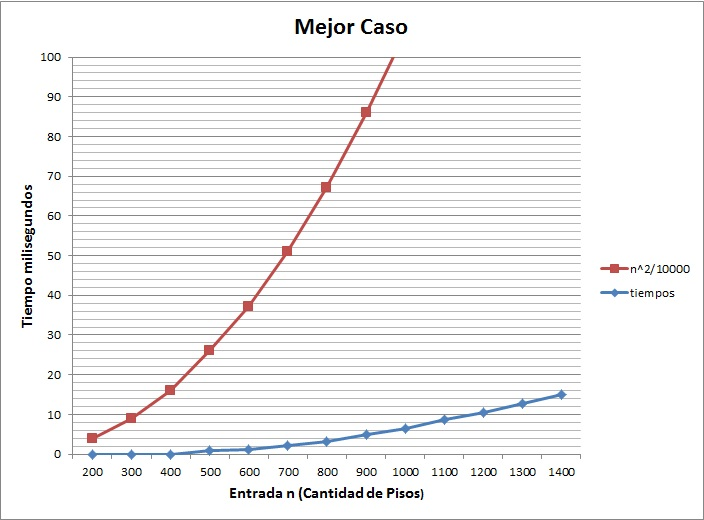
\includegraphics[scale=0.70]{imagenes/MejorCasoEj1.jpg}
	  \end{center}
 \caption{Mejor caso}
\end{figure}

Como la solución mínima de portales, es 1, dado un P fijo, ya que es un portal que va desde el primer hasta el ultimo piso, entonces la solución mas rápida que se puede hacer, es que haya un solo portal, ya que la matriz la vamos a recorrer en $O(n^2)$ y también vamos a agregar 1 portal ($O(n)$).

%\textbf{completar!}

%\newpage

Y nuestro "peor caso", también en base al mismo n fijo, es agregar la máxima cantidad de portales posibles, que es $n*(n-1)/2$, que seria agregar para $i<j<=n$, para cada piso $i=1,2,..,n$ un portal del piso $i$ hasta el piso $j$ con $j=i,i+1,..,n$. Entonces recorreríamos la matriz, en $O(n^2)$ y también la matriz, en $O(n*(n-1)/2)$ que queda en el mismo orden de $O(n^2)$ pero a la hora de la practica se nota una constante que los diferencia. 

\begin{figure}[H]
  \begin{center}
      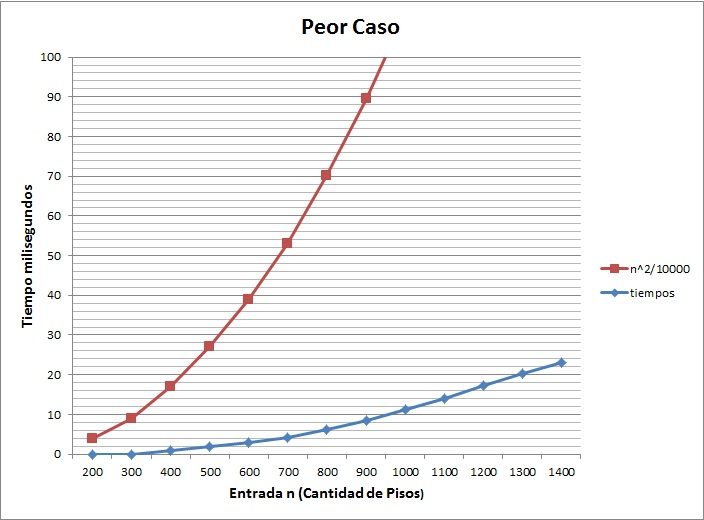
\includegraphics[scale=0.70]{imagenes/PeorCasoEj1.jpg}
	  \end{center}
 \caption{Peor Caso}
\end{figure}



\vspace*{0.3cm}

%\textbf{completar!}




%\newpage

%\vspace*{0.3cm}

%\textbf{completar!}

\begin{figure}[H]
  \begin{center}
      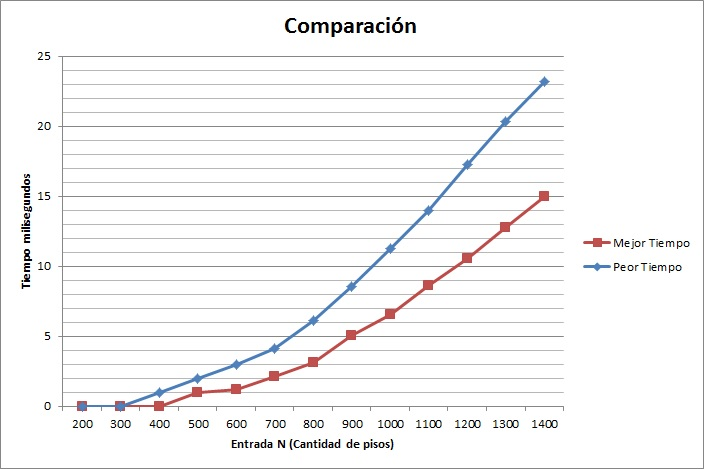
\includegraphics[scale=0.70]{imagenes/ComparacionEj1.jpg}
	  \end{center}
 \caption{Comparación entre el mejor y peor caso}
\end{figure}

Acá brindamos una comparación entre el mejor y  peor caso. aqui podemos notar que las mediciones empíricas de coinciden con lo teórico





%\newpage
%\subsubsection{Test 2}

%\vspace*{0.3cm}

%\textbf{completar!}


%\newpage
%\subsubsection{Test 3}

%\vspace*{0.3cm}

%\textbf{completar!}
